\documentclass[bachelor]{thesis-uestc}

\title{物联网脑机接口通信协议 Sudoku 的设计与实现}{Design and Implementation of Sudoku: An IoT BCI Communication Protocol}

% TODO: 替换为你的真实信息（敏感内容建议仅在 Gitea 分支维护）
\author{姓名}{Name}
\advisor{导师姓名\chinesespace 职称}{Supervisor Name}
\school{学院}{School}
\major{专业}{Major}
\studentnumber{学号}

% 图表：由 `cmd/iotbci-texgen` 生成的 pgfplots 片段
\usepackage{pgfplots}
\pgfplotsset{compat=1.18}

\begin{document}

\makecover

\begin{chineseabstract}
脑机接口（BCI）在物联网（IoT）场景下的局域网通信既需要低时延与低资源占用，也需要在面对主动探测、重放与中间人攻击时保持可靠的认证与抗侧写能力。本文围绕本仓库实现的 IoT\_BCI-Sudoku 协议，给出其握手认证、会话加密与 Sudoku 外观层（padding + 轮转/布局映射）的设计与工程实现，并通过与 DTLS / MQTT / CoAP / 纯 AEAD 封装的对比实验，展示其在“安全-效率-外观可辨识性”之间的权衡与适用边界。

\chinesekeyword{脑机接口，物联网，安全通信，抗重放，流量混淆，Sudoku}
\end{chineseabstract}

\begin{englishabstract}
Local-area communication for IoT BCI workloads requires low latency and low resource usage, while remaining robust against active probing, replay, and man-in-the-middle attacks. This thesis presents the design and implementation of the IoT\_BCI-Sudoku protocol in this repository, covering authenticated handshake, forward-secure session encryption, and a Sudoku-inspired appearance layer (padding and layout rotation/mapping). We also provide comparative evaluation against DTLS, MQTT, CoAP, and pure AEAD framing to characterize trade-offs among security, efficiency, and traffic fingerprintability.

\englishkeyword{BCI, IoT, secure communication, anti-replay, traffic obfuscation, Sudoku}
\end{englishabstract}

\thesistableofcontents

\chapter{绪论}
\section{研究背景与意义}
（TODO：结合开题报告完善。可参考本仓库 \texttt{doc/SECURITY.md} 与 \texttt{doc/OBFS\_SUDOKU.md}。）

\section{本文工作与结构}
本文主要工作包括：协议栈实现（握手/会话/外观层）、威胁模型与可复现实验工具、以及与 DTLS/MQTT/CoAP 等基线协议的量化对比。

\chapter{协议设计与实现}
\section{总体架构}
协议分层包括：握手认证（Ed25519 + X25519）、会话记录层（AEAD record）、以及外观层（Sudoku 映射与随机 padding）。实现细节参见 \texttt{doc/SPEC.md}、\texttt{doc/HANDSHAKE.md} 与源码 \texttt{pkg/iotbci}。

\section{Sudoku 外观层}
外观层通过将字节编码为 4 个 hint，并叠加可配置 padding，使得字节分布与长度分布不再固定，从而降低被动侧写与基于长度的指纹识别风险。

\chapter{威胁模型与安全分析}
\section{威胁模型}
本文考虑重放攻击、MITM、以及资源耗尽等威胁。详见 \texttt{doc/SECURITY.md}。

\section{工具模拟}
本仓库提供 \texttt{cmd/iotbci-attack} 用于在进程内模拟重放、篡改与探测洪泛等攻击，用于验证可疑路径与上层回落策略。

\chapter{性能评估与对比}
\section{实验方法}
本仓库提供 \texttt{cmd/iotbci-bench}（micro-bench）与 \texttt{cmd/iotbci-evidence}（回环 socket 证据集）。抓包侧写报告由 \texttt{cmd/iotbci-report} 生成，统一可视化由 \texttt{cmd/iotbci-dashboard} 生成。

\section{结果与分析}
表格与图表由 \texttt{cmd/iotbci-texgen} 自动生成（位于 \texttt{tex/generated}），可直接插入论文：

\IfFileExists{generated/bench_table.tex}{% Auto-generated by cmd/iotbci-texgen at 2026-01-31T11:48:22+08:00
\begin{table}[htbp]
\centering
\caption{Protocol comparison results (bench, auto-generated).}
\label{tab:iotbci-bench-metrics}
\begin{tabular}{lrrrrrrrr}
\toprule
Protocol & Overhead(x) & Avg RTT(ms) & P95 RTT(ms) & Wire(KB) & PeakHeap(MB) & WireTP(MB/s) & Entropy & ASCII\\
\midrule
coap-udp & 1.04 & 0.0496 & 0.0633 & 104.3 & 2.04 & 10.08 & 7.982 & 0.369\\
dtls-ecdhe-ecdsa-aes128gcm & 1.17 & 0.0827 & 0.1057 & 117.2 & 3.40 & 6.05 & 7.943 & 0.358\\
iotbci-sudoku-packed & 1.44 & 0.0151 & 0.0172 & 144.4 & 1.24 & 27.98 & 6.010 & 0.000\\
iotbci-sudoku-pure & 4.31 & 0.0400 & 0.0467 & 431.2 & 3.57 & 18.56 & 5.999 & 0.985\\
mqtt-3.1.1-qos0-tls & 2.82 & 0.0636 & 0.0995 & 282.1 & 2.79 & 19.61 & 7.926 & 0.350\\
pure-aead & 1.07 & 0.0136 & 0.0172 & 107.0 & 1.61 & 37.20 & 7.995 & 0.368\\
\bottomrule
\end{tabular}
\end{table}
}{\textit{(缺少 generated/bench\_table.tex，请先运行 cmd/iotbci-texgen 生成)}}

\IfFileExists{generated/bench_figures.tex}{% Auto-generated by cmd/iotbci-texgen at 2026-01-24T05:50:39+08:00
% Requires: \usepackage{pgfplots} and \pgfplotsset{compat=1.18}
\begin{figure}[htbp]
\centering
% Auto-generated by cmd/iotbci-texgen at 2026-01-24T05:50:39+08:00
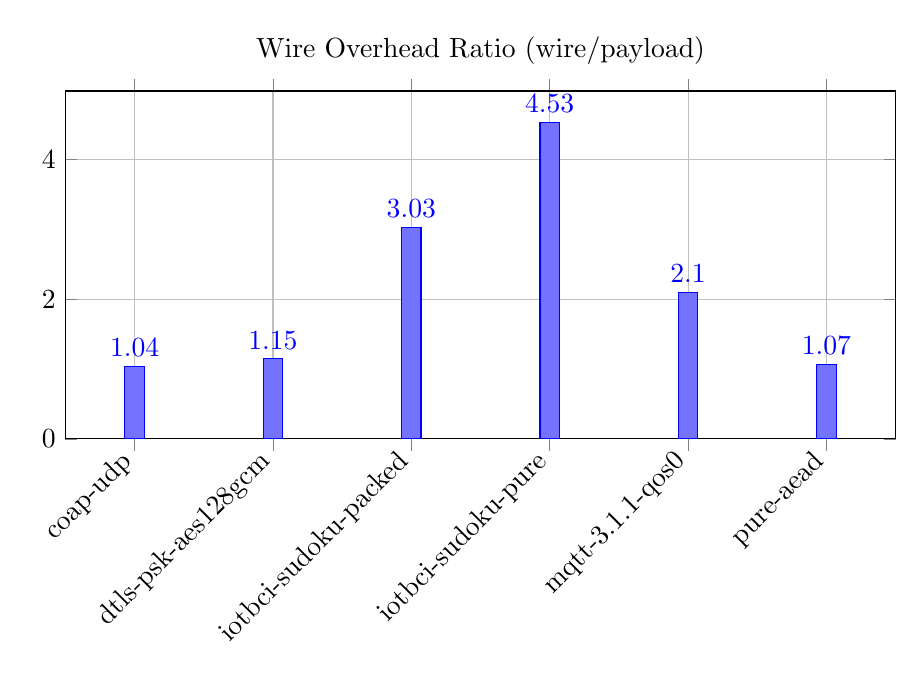
\begin{tikzpicture}
\begin{axis}[
  ybar,
  grid=major,
  width=\linewidth,
  height=6cm,
  ymin=0,
  title={Wire Overhead Ratio (wire/payload)},
  symbolic x coords={coap-udp,dtls-psk-aes128gcm,iotbci-sudoku-packed,iotbci-sudoku-pure,mqtt-3.1.1-qos0,pure-aead},
  xtick=data,
  x tick label style={rotate=45,anchor=east},
  bar width=7pt,
  nodes near coords,
  nodes near coords align={vertical},
]
\addplot+[fill=blue!55] coordinates {(coap-udp,1.042969) (dtls-psk-aes128gcm,1.145832) (iotbci-sudoku-packed,3.030416) (iotbci-sudoku-pure,4.530852) (mqtt-3.1.1-qos0,2.097826) (pure-aead,1.070312) };
\end{axis}
\end{tikzpicture}

\caption{Wire overhead ratio comparison (bench).}\label{fig:iotbci-bench-overhead}
\end{figure}

\begin{figure}[htbp]
\centering
% Auto-generated by cmd/iotbci-texgen at 2026-01-31T11:48:22+08:00
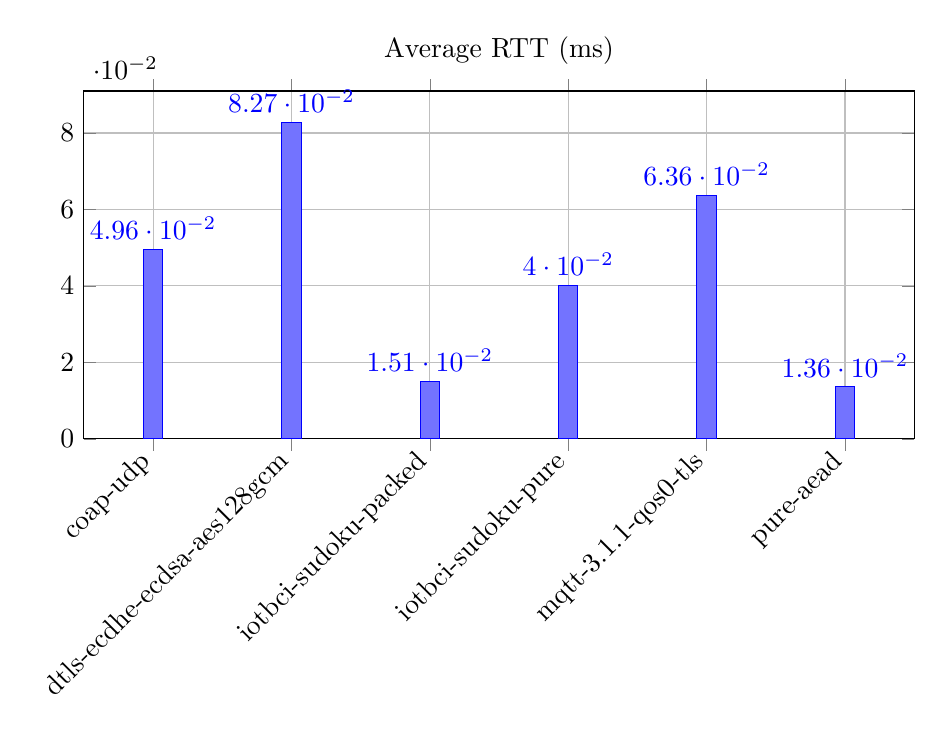
\begin{tikzpicture}
\begin{axis}[
  ybar,
  grid=major,
  width=\linewidth,
  height=6cm,
  ymin=0,
  title={Average RTT (ms)},
  symbolic x coords={coap-udp,dtls-ecdhe-ecdsa-aes128gcm,iotbci-sudoku-packed,iotbci-sudoku-pure,mqtt-3.1.1-qos0-tls,pure-aead},
  xtick=data,
  x tick label style={rotate=45,anchor=east},
  bar width=7pt,
  nodes near coords,
  nodes near coords align={vertical},
]
\addplot+[fill=blue!55] coordinates {(coap-udp,0.049579) (dtls-ecdhe-ecdsa-aes128gcm,0.082721) (iotbci-sudoku-packed,0.015051) (iotbci-sudoku-pure,0.040043) (mqtt-3.1.1-qos0-tls,0.063594) (pure-aead,0.013610) };
\end{axis}
\end{tikzpicture}

\caption{Average RTT comparison (bench).}\label{fig:iotbci-bench-rtt}
\end{figure}

\begin{figure}[htbp]
\centering
% Auto-generated by cmd/iotbci-texgen at 2026-01-24T05:50:39+08:00
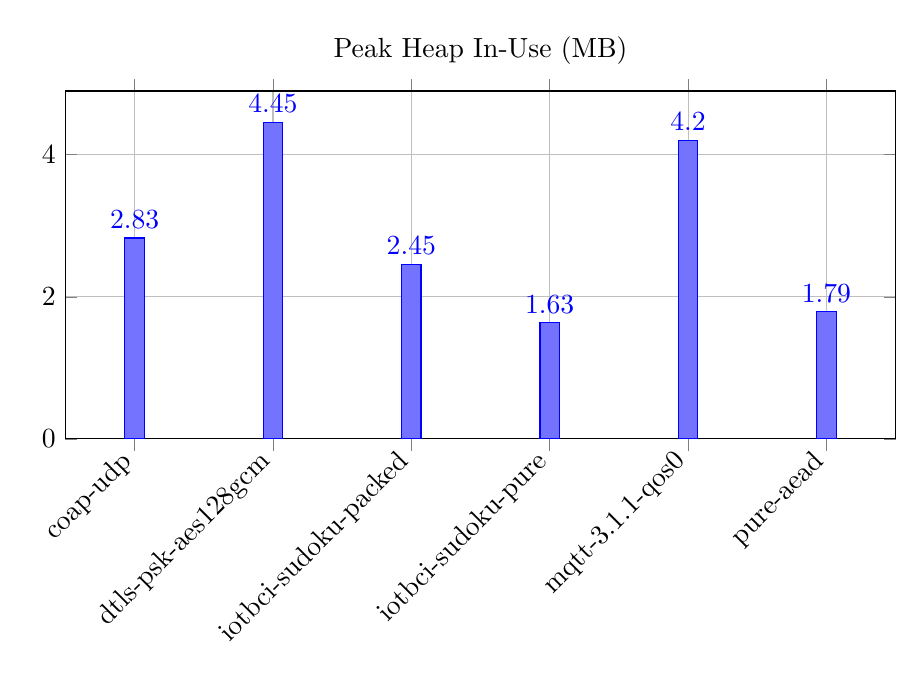
\begin{tikzpicture}
\begin{axis}[
  ybar,
  grid=major,
  width=\linewidth,
  height=6cm,
  ymin=0,
  title={Peak Heap In-Use (MB)},
  symbolic x coords={coap-udp,dtls-psk-aes128gcm,iotbci-sudoku-packed,iotbci-sudoku-pure,mqtt-3.1.1-qos0,pure-aead},
  xtick=data,
  x tick label style={rotate=45,anchor=east},
  bar width=7pt,
  nodes near coords,
  nodes near coords align={vertical},
]
\addplot+[fill=blue!55] coordinates {(coap-udp,2.828125) (dtls-psk-aes128gcm,4.453125) (iotbci-sudoku-packed,2.453125) (iotbci-sudoku-pure,1.632812) (mqtt-3.1.1-qos0,4.203125) (pure-aead,1.789062) };
\end{axis}
\end{tikzpicture}

\caption{Peak heap in-use comparison (bench).}\label{fig:iotbci-bench-mem}
\end{figure}

\begin{figure}[htbp]
\centering
% Auto-generated by cmd/iotbci-texgen at 2026-01-24T05:50:39+08:00
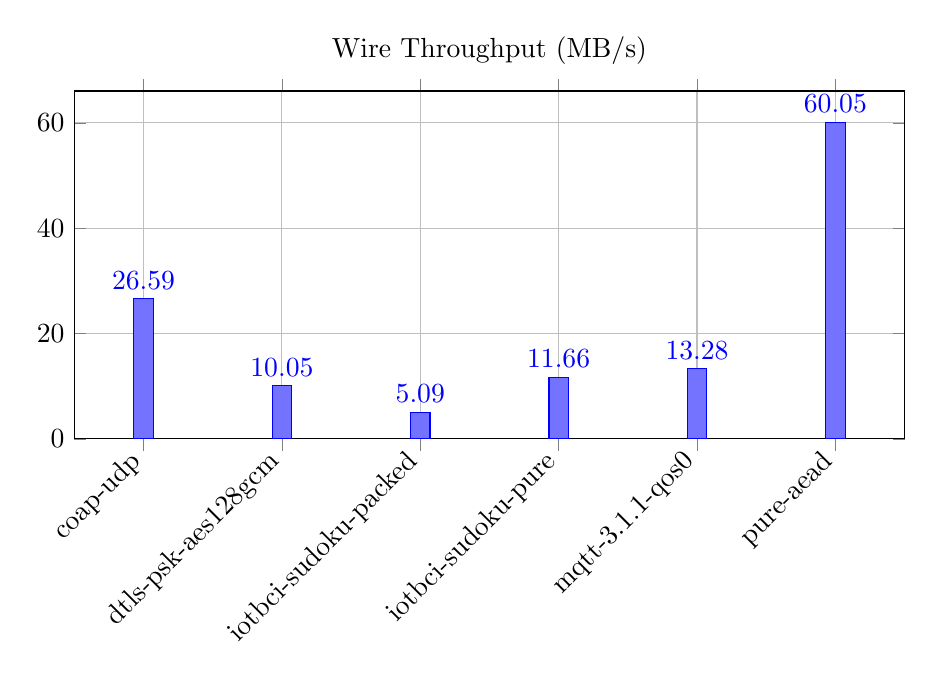
\begin{tikzpicture}
\begin{axis}[
  ybar,
  grid=major,
  width=\linewidth,
  height=6cm,
  ymin=0,
  title={Wire Throughput (MB/s)},
  symbolic x coords={coap-udp,dtls-psk-aes128gcm,iotbci-sudoku-packed,iotbci-sudoku-pure,mqtt-3.1.1-qos0,pure-aead},
  xtick=data,
  x tick label style={rotate=45,anchor=east},
  bar width=7pt,
  nodes near coords,
  nodes near coords align={vertical},
]
\addplot+[fill=blue!55] coordinates {(coap-udp,26.593320) (dtls-psk-aes128gcm,10.052351) (iotbci-sudoku-packed,5.090040) (iotbci-sudoku-pure,11.664659) (mqtt-3.1.1-qos0,13.279945) (pure-aead,60.054706) };
\end{axis}
\end{tikzpicture}

\caption{Wire throughput comparison (bench).}\label{fig:iotbci-bench-throughput}
\end{figure}

\begin{figure}[htbp]
\centering
% Auto-generated by cmd/iotbci-texgen at 2026-01-24T05:50:39+08:00
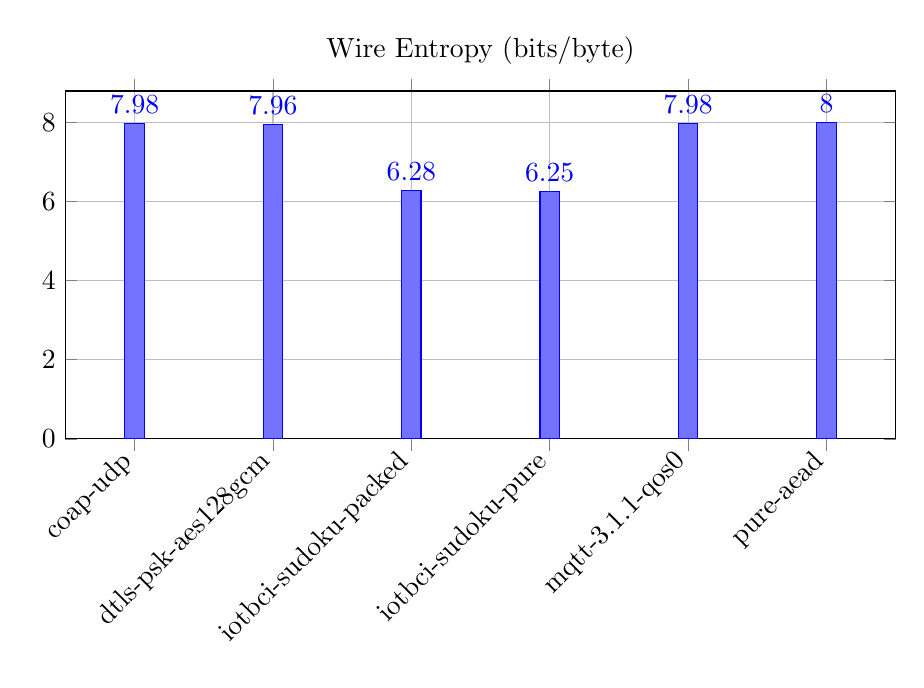
\begin{tikzpicture}
\begin{axis}[
  ybar,
  grid=major,
  width=\linewidth,
  height=6cm,
  ymin=0,
  title={Wire Entropy (bits/byte)},
  symbolic x coords={coap-udp,dtls-psk-aes128gcm,iotbci-sudoku-packed,iotbci-sudoku-pure,mqtt-3.1.1-qos0,pure-aead},
  xtick=data,
  x tick label style={rotate=45,anchor=east},
  bar width=7pt,
  nodes near coords,
  nodes near coords align={vertical},
]
\addplot+[fill=blue!55] coordinates {(coap-udp,7.980901) (dtls-psk-aes128gcm,7.956253) (iotbci-sudoku-packed,6.281114) (iotbci-sudoku-pure,6.247452) (mqtt-3.1.1-qos0,7.978827) (pure-aead,7.995770) };
\end{axis}
\end{tikzpicture}

\caption{Wire entropy comparison (bench).}\label{fig:iotbci-bench-entropy}
\end{figure}

\begin{figure}[htbp]
\centering
% Auto-generated by cmd/iotbci-texgen at 2026-01-24T05:50:39+08:00
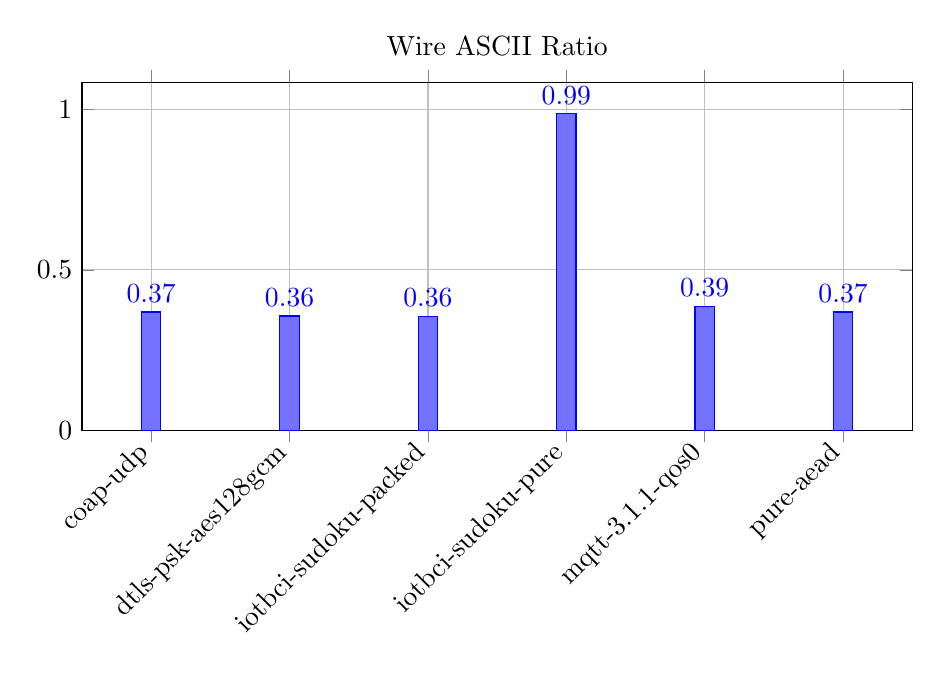
\begin{tikzpicture}
\begin{axis}[
  ybar,
  grid=major,
  width=\linewidth,
  height=6cm,
  ymin=0,
  title={Wire ASCII Ratio},
  symbolic x coords={coap-udp,dtls-psk-aes128gcm,iotbci-sudoku-packed,iotbci-sudoku-pure,mqtt-3.1.1-qos0,pure-aead},
  xtick=data,
  x tick label style={rotate=45,anchor=east},
  bar width=7pt,
  nodes near coords,
  nodes near coords align={vertical},
]
\addplot+[fill=blue!55] coordinates {(coap-udp,0.368464) (dtls-psk-aes128gcm,0.355867) (iotbci-sudoku-packed,0.355310) (iotbci-sudoku-pure,0.986572) (mqtt-3.1.1-qos0,0.385478) (pure-aead,0.368378) };
\end{axis}
\end{tikzpicture}

\caption{Wire ASCII ratio comparison (bench).}\label{fig:iotbci-bench-ascii}
\end{figure}

\begin{figure}[htbp]
\centering
% Auto-generated by cmd/iotbci-texgen at 2026-01-31T11:48:22+08:00
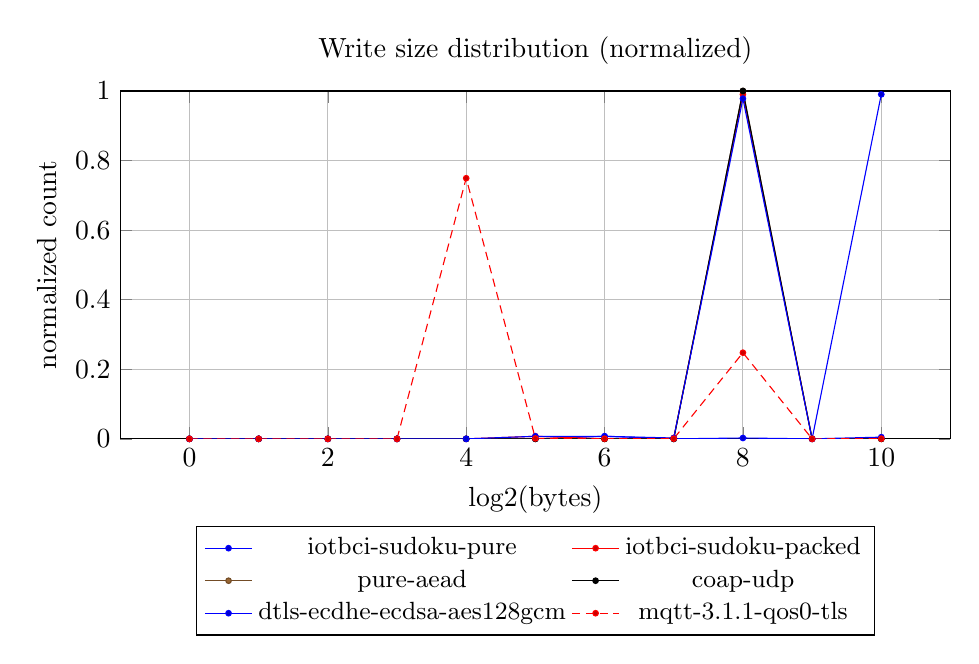
\begin{tikzpicture}
\begin{axis}[
  grid=major,
  width=\linewidth,
  height=6cm,
  ymin=0,
  ymax=1,
  title={Write size distribution (normalized)},
  xlabel={log2(bytes)},
  ylabel={normalized count},
  legend style={font=\small, at={(0.5,-0.25)}, anchor=north, legend columns=2},
]
% Each series is normalized by its own total count.
% maxBin=10, metric=write\_size
\addplot+[mark=*,mark size=1pt] coordinates {(0,0.000000) (1,0.000000) (2,0.000000) (3,0.000000) (4,0.000000) (5,0.000000) (6,0.007389) (7,0.000000) (8,0.002463) (9,0.000000) (10,0.990148) };
\addlegendentry{iotbci-sudoku-pure}
\addplot+[mark=*,mark size=1pt] coordinates {(0,0.000000) (1,0.000000) (2,0.000000) (3,0.000000) (4,0.000000) (5,0.007389) (6,0.000000) (7,0.002463) (8,0.990148) (9,0.000000) (10,0.000000) };
\addlegendentry{iotbci-sudoku-packed}
\addplot+[mark=*,mark size=1pt] coordinates {(0,0.000000) (1,0.000000) (2,0.000000) (3,0.000000) (4,0.000000) (5,0.000000) (6,0.000000) (7,0.000000) (8,1.000000) (9,0.000000) (10,0.000000) };
\addlegendentry{pure-aead}
\addplot+[mark=*,mark size=1pt] coordinates {(0,0.000000) (1,0.000000) (2,0.000000) (3,0.000000) (4,0.000000) (5,0.000000) (6,0.000000) (7,0.000000) (8,1.000000) (9,0.000000) (10,0.000000) };
\addlegendentry{coap-udp}
\addplot+[mark=*,mark size=1pt] coordinates {(0,0.000000) (1,0.000000) (2,0.000000) (3,0.000000) (4,0.000000) (5,0.007335) (6,0.007335) (7,0.002445) (8,0.977995) (9,0.000000) (10,0.004890) };
\addlegendentry{dtls-ecdhe-ecdsa-aes128gcm}
\addplot+[mark=*,mark size=1pt] coordinates {(0,0.000000) (1,0.000000) (2,0.000000) (3,0.000000) (4,0.749226) (5,0.001238) (6,0.000619) (7,0.000619) (8,0.247678) (9,0.000000) (10,0.000619) };
\addlegendentry{mqtt-3.1.1-qos0-tls}

\end{axis}
\end{tikzpicture}

\caption{Write size distribution (appearance metric, bench).}\label{fig:iotbci-bench-write-size}
\end{figure}

\begin{figure}[htbp]
\centering
\input{generated/bench_write_iat_plot}
\caption{Write inter-arrival distribution (appearance metric, bench).}\label{fig:iotbci-bench-write-iat}
\end{figure}
}{\textit{(缺少 generated/bench\_figures.tex，请先运行 cmd/iotbci-texgen 生成)}}

\chapter{总结与展望}
（TODO：总结结论，并结合进度计划补充后续工作：端侧资源上限参数化、证书吊销/轮换、以及更完整的抓包侧写与攻击自动化验证。）

\thesisbibliography{reference}

\end{document}
